\documentclass[UTF8,a4paper,11pt]{ctexart}

\usepackage{geometry}
\usepackage{amsmath,amssymb,bm}
\usepackage{graphicx}
\usepackage{booktabs}
\usepackage{tabularx}
\usepackage{longtable}
\usepackage{array}
\usepackage{enumitem}
\usepackage{xcolor}
\usepackage{hyperref}

\geometry{left=2.5cm,right=2.5cm,top=2.6cm,bottom=2.6cm}
\hypersetup{
  colorlinks=true,
  linkcolor=black,
  citecolor=black,
  urlcolor=blue
}
\setlist[itemize]{leftmargin=2em,itemsep=0.2em,topsep=0.2em}
\setlist[enumerate]{leftmargin=2em,itemsep=0.2em,topsep=0.2em}
\renewcommand{\arraystretch}{1.15}
\emergencystretch=2em

\newcolumntype{Y}{>{\raggedright\arraybackslash}X}
\newcommand{\mae}{\mathrm{MAE}}
\newcommand{\rmse}{\mathrm{RMSE}}
\newcommand{\rdsq}{R^2}
\newcommand{\ev}{\mathrm{eV}}
\newcommand{\NA}{--}

\title{\bfseries 基于 ALIGNN 全局虚拟节点增强的晶体带隙预测及 MP--HZW 标签一致性分析}
\author{项目论文初稿}
\date{2026 年 6 月 11 日}

\begin{document}

\maketitle

\begin{abstract}
晶体带隙预测是计算材料发现中的核心回归任务。图神经网络能够直接利用原子种类、晶格、周期近邻和局部几何信息，但局部消息传递模型可能受到全局信息汇聚不足的限制；同时，不同材料数据库中的 band gap 标签并不总是等价，这会显著影响模型排序和结论解释。本文系统整理了一个围绕晶体 band gap 预测的 GNN 实验谱系：首先复现并比较 CGCNN、ALIGNN 和 M3GNet 等基线模型；随后在 ALIGNN 上引入朴素 virtual node、全局注意力、物理约束、双槽位 virtual node、size-supervised gate 等增强机制；最后在 MP--HZW structure-first audit 后构建 relaxed clean equal-atoms 双标签源数据集，并完成 Huber loss、top-$k$ 汇聚、warmup top-$k$ 与 global broadcast decay 的消融验证。实验表明，在早期 HZW 口径下，E4 朴素 virtual node 已稳定优于 ALIGNN baseline，E12/E13 双槽位与物理约束进一步取得历史最优；但在 MP full 与后续 matched 数据上，复杂全局槽位并未稳定超过单 virtual node。最终 relaxed clean equal-atoms 口径下，MP label 中 T10 获得最低 MAE 0.223686，HZW label 中 T7 获得最低 MAE 0.194002。跨两个标签源最稳健的结论是：ALIGNN + single plain virtual node + Huber loss 带来稳定收益；top-$k$ 与双节点机制具有数据源依赖，不能作为当前主贡献。本文进一步说明，结构匹配与标签一致性必须分开审计，材料 GNN 的模型比较应严格标注数据口径与标签来源。
\end{abstract}

\noindent\textbf{关键词：}晶体图神经网络；带隙预测；ALIGNN；虚拟节点；Huber loss；Materials Project；数据一致性

\section{引言}

带隙（band gap）决定材料的金属、半导体或绝缘体属性，是光伏、电子器件、催化和能源材料筛选中的关键物性。传统第一性原理计算能够提供高质量电子结构估计，但在大规模材料搜索中计算成本较高。近年来，晶体图神经网络通过把晶体结构表示为周期图，在原子节点、键边、晶格和局部几何之间进行消息传递，已成为材料性质预测的重要方法。

本项目关注一个具体问题：在晶体 band gap 回归任务上，ALIGNN 这类局部几何 GNN 是否需要额外的全局信息通道？如果需要，简单的 virtual node、复杂全局注意力、双槽位机制、物理约束和鲁棒损失各自贡献是什么？这一问题并不只是模型结构问题。项目早期在 HZW bandgap 标签上观察到双槽位和物理约束的积极信号，但迁移到 Materials Project（MP）summary band\_gap 后，模型排序发生变化。因此，本文同时研究模型增强和跨标签源数据一致性。

本文贡献概括为三点。第一，系统复现并比较 CGCNN、ALIGNN、M3GNet 及 E1--E13 多种 ALIGNN 全局增强模型，确认 ALIGNN + 朴素 virtual node 是稳定强基线。第二，通过 MP--HZW structure-first audit 证明结构匹配与标签一致性必须分开处理，揭示两个 band gap 标签源存在金属/非金属冲突和大幅数值差异。第三，在 relaxed clean equal-atoms 双标签源上完成 T 系列消融，发现 Huber loss 是跨标签源最稳定的进一步收益来源，而 top-$k$、双节点和复杂路由机制具有明显数据源依赖。

本文结论保持谨慎：在当前实验口径下，最可靠的主模型不是最复杂的双槽位或 top-$k$ 模型，而是 ALIGNN + single plain virtual node + Huber loss。MP label 上 global broadcast decay 的 T10 进一步取得最低 MAE，但该收益没有在 HZW label 上同等保持，因此更适合作为 MP label 特化改进，而非跨源通用结论。

\section{相关工作}

\subsection{晶体图神经网络}

CGCNN 将晶体表示为原子图，通过卷积消息传递学习局部化学环境，是晶体性质预测的早期代表模型\cite{xie2018cgcnn}。ALIGNN 进一步在 atom graph 之外构造 line graph，使模型能够显式利用键角和二阶几何关系，在多项材料性质预测任务中表现强劲\cite{choudhary2021alignn}。M3GNet 则从通用材料图势能模型角度出发，引入三体几何信息，并展示了跨元素周期表的泛化能力\cite{chen2022m3gnet}。本项目把 ALIGNN 作为主要骨架，因为它在早期 HZW 和后续 MP 口径中均是最强传统 baseline。

\subsection{全局信息建模与 virtual node}

局部消息传递 GNN 的一个常见瓶颈是远距离信息需要多层传播才能交互，深层堆叠又可能导致过平滑或训练困难。Virtual node 通过引入一个全图级 token，在每层从所有原子节点汇聚信息并向节点广播，为模型提供低成本的全局通道。与直接堆叠 Transformer 或全局 attention 相比，朴素 virtual node 的归纳偏置更简单，也更容易保持与局部几何消息传递的互补关系。本文的 E4、T4 和 T7 均以这一思路为核心。

\subsection{物理约束、鲁棒损失与材料数据集}

材料物性预测常结合物理先验，例如利用 CBM/VBM 与 band gap 的一致性进行辅助监督，或在损失函数中引入非负约束。另一方面，band gap 标签通常存在方法误差、数据库版本差异和金属/非金属边界不一致。Huber loss 在小误差区间近似 MSE、在大误差区间近似 MAE，适合在存在异常标签或重尾噪声时降低极端样本对训练的破坏。本文最终 T 系列的关键发现正是 Huber loss 在 MP label 和 HZW label 两个口径上都带来稳定收益。

Materials Project 是材料数据与计算材料发现的重要公共资源\cite{jain2013mp}。Matbench 为材料性质预测提供了标准化 benchmark 视角\cite{dunn2020matbench}。然而，本文处理的 HZW 与 MP matched 数据说明，即使结构可以匹配，band gap 标签也可能来自不同处理流程或版本，因此不能把结构对应直接等同为标签等价。

\section{数据与审计}

\subsection{任务定义与评价指标}

主任务是晶体结构到 band gap 的回归预测，单位为 eV。输入包括原子种类、坐标、晶格和周期近邻关系；ALIGNN 系列模型额外使用 line graph 表示键角和二阶几何。主指标为测试集 MAE，辅助指标包括 RMSE、$\rdsq$、Metal F1、best epoch、训练耗时和峰值显存。Metal F1 由预测带隙与标签带隙的金属/非金属判别导出，用于观察模型是否改善 0-gap 边界附近的分类表现。

\subsection{数据阶段与口径}

表\ref{tab:data-stages}总结了本文涉及的数据阶段。需要强调的是，这些数据阶段不能直接混合比较。早期 HZW 结果用于解释模型设计演化；MP full 用于公开 MP bandgap 泛化诊断；strict clean S 系列用于双节点分桶诊断；relaxed clean equal-atoms 才是最终 T 系列主口径。

\begin{table}[htbp]
\centering
\caption{数据阶段与可比较口径。}
\label{tab:data-stages}
\scriptsize
\begin{tabularx}{\textwidth}{p{3.0cm} p{2.2cm} p{3.0cm} Y}
\toprule
阶段 & 样本/记录口径 & 用途 & 写作注意事项 \\
\midrule
HZW 原始 bandgap & 约 95,497 & E1--E13 早期实验 & E4、E12、E13 在 HZW 上有效，但不能与最终 T 系列直接数值比较。 \\
MP full & 约 154,875 & 公开 MP bandgap 泛化 & E4 重新最稳，复杂双槽位未稳定超过 E4。 \\
MP--HZW structure-first audit & 总 95,462；结构匹配 92,787；缺 MP 2,636；结构不匹配 39 & 区分结构匹配和标签一致性 & 结构匹配不等于 band gap 标签一致。 \\
strict clean MP-label & accepted 81,751；test 8,176 & S 系列严格清洗 & 删除 gap 差值和体积差过大的版本，后续不作为最终主口径。 \\
relaxed clean equal-atoms MP label & accepted 84,550；train/val/test = 67,640/8,455/8,455 & 最终 T 系列 MP 标签口径 & 不删除大 gap 差值和大体积差，只删除零/非零冲突与原子数非 equal。 \\
relaxed clean equal-atoms HZW label & accepted 84,550；train/val/test = 67,640/8,455/8,455 & 最终 T 系列 HZW 标签口径 & 同一批结构，替换为 HZW bandgap 标签。 \\
\bottomrule
\end{tabularx}
\end{table}

\subsection{MP--HZW structure-first audit}

MP--HZW 审计采用 structure-first 思路：先判断 MP 与 HZW 晶体结构是否对应，再在结构匹配样本内部统计标签冲突。最终锁定的审计结果见表\ref{tab:audit-counts}。在 95,462 条可审计记录中，92,787 条结构匹配，其中 92,507 条为 exact match，280 条为 supercell match；39 条结构不匹配，2,636 条缺少 MP 记录。

\begin{table}[htbp]
\centering
\caption{MP--HZW structure-first audit 关键计数。}
\label{tab:audit-counts}
\small
\begin{tabular}{l r}
\toprule
项目 & 数量 \\
\midrule
Total rows & 95,462 \\
Structure matched rows & 92,787 \\
Structure unmatched rows & 39 \\
Compatible but unverified rows & 0 \\
Missing MP records & 2,636 \\
\midrule
\texttt{structure\_matched\_exact} & 92,507 \\
\texttt{structure\_matched\_supercell} & 280 \\
\bottomrule
\end{tabular}
\end{table}

在结构匹配样本内部，标签冲突仍然显著。表\ref{tab:label-conflict}显示，85,478 条没有标签冲突，但仍有 3,142 条属于 MP metal / HZW nonmetal，3,046 条属于 MP nonmetal / HZW metal，另有 1,121 条同类样本的 band gap 差异超过 1 eV。这些冲突足以改变回归损失、Metal F1 和模型排序。

\begin{table}[htbp]
\centering
\caption{结构匹配样本内部的标签冲突。}
\label{tab:label-conflict}
\small
\begin{tabular}{l r}
\toprule
类型 & 数量 \\
\midrule
\texttt{no\_label\_conflict} & 85,478 \\
\texttt{mp\_metal\_hzw\_nonmetal} & 3,142 \\
\texttt{mp\_nonmetal\_hzw\_metal} & 3,046 \\
\texttt{same\_class\_gap\_diff\_gt\_1ev} & 1,121 \\
\bottomrule
\end{tabular}
\end{table}

\subsection{relaxed clean equal-atoms 规则}

最终 T 系列采用 relaxed clean equal-atoms 口径。从 92,787 条结构匹配样本出发，删除 band gap 零/非零金属边界冲突 7,984 条，删除 \texttt{atom\_count\_relation != equal} 的 252 条；不再删除 $\lvert \mathrm{mp\_gap}-\mathrm{hzw\_gap}\rvert > 0.5\ev$ 的样本，也不再删除 \texttt{volume\_per\_atom\_rel\_diff > 8\%} 的样本。最终 accepted records 为 84,550 条，并在同一结构划分上分别使用 MP label 和 HZW label 训练 T 系列。

这个口径的优点是保留了更多结构匹配样本，同时排除了最直接破坏金属/非金属边界的零/非零冲突。其局限是仍保留同类但数值差异较大的标签，因此最终结论需要配合 Huber loss 与跨标签源验证解释。

\section{方法}

\subsection{基线模型}

E1/T1 为 CGCNN baseline，E2/T2 为 ALIGNN baseline，E3/T3 为 M3GNet baseline。CGCNN 主要在原子图上做局部消息传递；ALIGNN 同时在 atom graph 与 line graph 上传播，以捕获键角几何；M3GNet 使用材料图神经网络和三体几何。早期实验显示，ALIGNN 是本项目中最强传统 baseline，因此后续可引用主线主要围绕 ALIGNN 改造。

\subsection{朴素 virtual node}

E4/T4 在 ALIGNN 上加入 single plain virtual node。第 $l$ 层中，模型先从原子节点集合汇聚全局 token：
\begin{equation}
\mathbf{g}^{(l)}=\mathrm{Pool}\left(\{\mathbf{h}_i^{(l)}\}_{i=1}^{n}\right),
\end{equation}
再将全局上下文广播回每个原子节点：
\begin{equation}
\mathbf{h}_i^{(l+1)}
= \mathrm{ALIGNNLayer}(\mathbf{h}_i^{(l)},\mathcal{G})
+ \phi(\mathbf{g}^{(l)}).
\end{equation}
这一设计不依赖显式 size 特征或复杂 attention，是后续所有稳定改进的核心主干。

\subsection{物理约束}

E6 在 ALIGNN 主干上加入 CBM/VBM 辅助监督与 band gap 一致性约束。E13 在 E12 双槽位基础上进一步加入同类物理项。总损失可写为
\begin{equation}
L = L_{\mathrm{gap}} + \lambda_{\mathrm{aux}}L_{\mathrm{CBM/VBM}}
+ \lambda_{\mathrm{phys}}L_{\mathrm{gap=CBM-VBM}}
+ \lambda_{\mathrm{nonneg}}L_{\mathrm{nonneg}}.
\end{equation}
对于缺失或无效 CBM/VBM 的样本，使用有效 mask：
\begin{equation}
m_i = \mathbb{1}\left(|\mathrm{CBM}_i|>\epsilon \lor |\mathrm{VBM}_i|>\epsilon\right),
\end{equation}
只在 $m_i=1$ 的样本上计算辅助物理损失，避免把缺失值误当成物理信号。

\subsection{双槽位与 size-supervised gate}

E7/E8 将朴素 virtual node 替换或扩展为 attentive virtual node。E7 使用单 attentive slot，E8 使用两个 attentive slots 并加入 slot 间交互。早期 HZW 分桶结果显示 E8 在大结构上优于 E4，因此 E12 进一步保留一个稳定主 slot，并加入第二个可门控 slot。E12 的关键设计是：\texttt{num\_atoms} 不进入前向 gate 输入，只在训练损失中构造软标签监督第二槽位开启程度。其动机是鼓励模型在大结构中使用额外全局容量，同时避免推理时直接依赖手工 size 特征。

MP full 结果后来表明，这一代理变量具有数据源依赖。MP 上 \texttt{num\_atoms} 并不是“需要第二全局槽位”的稳定代理，导致 E7/E8/E12 均未稳定超过 E4。

\subsection{Huber loss}

T7 将 T4 的最终 band gap 回归损失由 MSE 替换为 Huber loss：
\begin{equation}
L_{\delta}(e)=
\begin{cases}
\frac{1}{2}e^2, & |e|\le \delta,\\
\delta(|e|-\frac{1}{2}\delta), & |e|>\delta.
\end{cases}
\end{equation}
其中 $e=\hat{y}-y$。小误差区间保留 MSE 的精细拟合能力，大误差区间降低异常标签或强冲突样本的梯度影响。最终 T 系列表明，Huber-only 是跨 MP label 与 HZW label 最稳定的进一步提升。

\subsection{Top-$k$、warmup 与 broadcast decay}

T6 在 T4 上同时加入 top-$k$ node-to-global 汇聚和 Huber loss。Top-$k$ 汇聚先计算节点得分 $s_i$，选择
\begin{equation}
\mathcal{K}=\mathrm{TopK}(s_i,k),\quad
\mathbf{g}=\sum_{i\in\mathcal{K}}\alpha_i\mathbf{h}_i,
\end{equation}
其中 $k=\mathrm{clip}(\lceil0.2n\rceil,k_{\min},k_{\max})$。T8 是 top-$k$ only 消融，保持 MSE；T9 使用 warmup top-$k$：
\begin{equation}
\mathbf{g}_{\mathrm{update}}=
(1-\alpha_t)\mathbf{g}_{\mathrm{mean}}+\alpha_t\mathbf{g}_{\mathrm{topk}},
\end{equation}
训练前期使用 mean pooling，中期线性增大 $\alpha_t$，后期使用 top-$k$。

T10 则从 global-to-node 方向调整信息流，在 Huber 和 single virtual node 主干上加入 broadcast decay：
\begin{equation}
\mathbf{h}_i^{(l+1)}
= \mathrm{ALIGNNLayer}(\mathbf{h}_i^{(l)},\mathcal{G})
+ \gamma_t\phi(\mathbf{g}^{(l)}).
\end{equation}
训练后期逐步降低 $\gamma_t$，以减少全局 token 对局部节点表示的噪声注入。T10 在 MP label 上最优，但在 HZW label 上不如 T7，说明该策略存在数据源依赖。

\section{实验设置}

\subsection{实验编号}

本文使用三组编号。E 系列表示早期主线与后续机制探索；S 系列表示 strict clean MP label 上的双节点诊断；T 系列表示 relaxed clean equal-atoms 最终口径。需要注意，早期 E13 表示 ``E12 + physics''，而后期 \texttt{configs/mp/MP\_E13\_alignn\_plain\_dual\_virtualnode.yaml} 实际是 plain dual virtual node 模板，在本文中称为 S13 或 T5，避免与早期 E13 混淆。

\subsection{训练与评价}

所有可比较结果均使用对应数据口径的固定 train/validation/test 划分。主结果以 test MAE 排序，RMSE、$\rdsq$、Metal F1 和 best epoch 用于辅助解释。早期 HZW 与 MP full 结果来自项目历史报告与实现汇总；structure-first audit 结果来自 \texttt{results/data\_quality/structure\_first\_strict\_180/}；S 系列分桶结果来自 \texttt{results/mp\_hzw\_final\_clean\_equal\_atoms\_mp\_s/analysis/}；最终 T 系列数值来自 2026-06-11 交付计划中已核对的远端 \texttt{comparison\_summary.csv}。

\section{结果}

\subsection{HZW 早期 E1--E13 主线}

表\ref{tab:hzw-early}展示 HZW 早期核心结果。E2 ALIGNN 明显优于 E1 CGCNN 和 E3 M3GNet，是最强传统 baseline。E4 在 ALIGNN 上加入朴素 virtual node 后，MAE 从 0.231432 降至 0.220077，Metal F1 也提升至 0.883811，说明简单全局汇聚有效。E6 的 MAE 略高于 E4，但 RMSE 和 $\rdsq$ 最优，说明物理约束改善了误差分布稳定性。E12 和 E13 进一步在 HZW 上超过 E4，其中 E13 达到 MAE 0.211944，是 HZW 早期历史最优。

\begin{table}[htbp]
\centering
\caption{HZW 早期核心实验结果。该表用于解释模型设计演化，不与最终 T 系列直接横向比较。}
\label{tab:hzw-early}
\small
\begin{tabular}{l l r r r r}
\toprule
实验 & 模型 & MAE & RMSE & $\rdsq$ & 结论 \\
\midrule
E1 & CGCNN & 0.302169 & 0.530287 & 0.884731 & 基础 baseline \\
E2 & ALIGNN & 0.231432 & 0.471325 & 0.908939 & 最强传统 baseline \\
E3 & M3GNet & 0.268041 & 0.553444 & 0.874444 & 材料图 baseline \\
E4 & ALIGNN + VN & 0.220077 & 0.474616 & 0.907663 & 朴素超节点有效 \\
E5 & ALIGNN + Transformer & 0.237450 & 0.491768 & 0.900869 & 全局注意力 only 不稳 \\
E6 & ALIGNN + physics & 0.221208 & 0.453924 & 0.915539 & RMSE/$\rdsq$ 更稳 \\
E8 & 2 attentive VN & 0.228456 & 0.494547 & 0.899745 & 大结构有信号 \\
E12 & size-supervised dual slot & 0.217873 & 0.471199 & 0.908988 & HZW 上超过 E4 \\
E13 & E12 + physics & \textbf{0.211944} & 0.461645 & 0.912641 & HZW 历史最优 \\
\bottomrule
\end{tabular}
\end{table}

HZW 分桶结果解释了为什么项目曾转向双槽位路线。E4 在 $\leq80$ 原子的桶中最稳，而 E8 在 81--160 和 $>160$ 原子桶中分别达到 0.3736 和 0.2696，优于 E4 的 0.3796 和 0.2930。这说明额外全局容量在大结构上可能有局部价值，但该观察随后需要在其他标签源上验证。

\subsection{MP full 与 matched clean：复杂槽位收益不稳}

迁移到 MP full 后，E4 重新成为最优模型。表\ref{tab:mp-full}显示，E4 MAE 为 0.230159，优于 E7、E8 和 E12。这个结果否定了“模型越复杂越好”的简单解释，也说明 HZW 上 ``size $\rightarrow$ second slot'' 的假设不能直接迁移到 MP label。

\begin{table}[htbp]
\centering
\caption{MP full 复现结果。}
\label{tab:mp-full}
\small
\begin{tabular}{l l r r r r}
\toprule
实验 & 模型 & MAE & RMSE & $\rdsq$ & Best Epoch \\
\midrule
E2 & ALIGNN & 0.239663 & \NA & \NA & \NA \\
E4 & ALIGNN + VN & \textbf{0.230159} & \textbf{0.512199} & \textbf{0.885399} & 50 \\
E7 & 1 attentive VN & 0.239001 & 0.527332 & 0.878527 & 48 \\
E8 & 2 attentive VN & 0.241759 & 0.526103 & 0.879093 & 43 \\
E12 & size-supervised & 0.236332 & 0.518681 & 0.882480 & 48 \\
\bottomrule
\end{tabular}
\end{table}

在后续 MP--HZW matched clean 结果中，E4 仍然是最稳模型：E2 MAE 为 0.2534，E4 为 0.2446，E8 为 0.2476，E10 验证集路由为 0.2455。硬阈值路由并不鲁棒，因为验证集阈值不能稳定迁移到测试集。这些结果共同说明，复杂全局注意力和双槽位并未在 MP summary band\_gap 监督目标下形成稳定收益。

\subsection{S 系列：双朴素节点有大结构信号但整体不赢}

Strict clean MP label 的 S 系列用于诊断 plain dual virtual node 是否能在大结构上发挥作用。表\ref{tab:s-series}显示，S13 在 81--160、$>160$ 和合并 $>80$ 子集上优于 S4，但整体 MAE 为 0.201181，略差于 S4 的 0.200094。其主要损失来自样本数较多的 21--40 与 41--80 桶，抵消了大结构收益。

\begin{table}[htbp]
\centering
\caption{Strict clean MP label 中 S4 与 S13 的分桶诊断。该结果说明双节点有局部信号，但不是稳定主模型。}
\label{tab:s-series}
\small
\begin{tabular}{l r r r r l}
\toprule
原子数桶 & 样本数 & mean atoms & S4 MAE & S13 MAE & winner \\
\midrule
$\leq10$ & 2,327 & 6.003 & 0.118300 & 0.118845 & S4 \\
11--20 & 1,873 & 15.601 & 0.175596 & 0.172570 & S13 \\
21--40 & 2,106 & 29.986 & 0.235496 & 0.243521 & S4 \\
41--80 & 1,452 & 57.574 & 0.279100 & 0.280506 & S4 \\
81--160 & 369 & 106.488 & 0.321578 & 0.307066 & S13 \\
$>160$ & 27 & 190.333 & 0.278618 & 0.266599 & S13 \\
\midrule
Overall & 8,154 & \NA & \textbf{0.200094} & 0.201181 & S4 \\
$>80$ 合并 & 396 & 112.205 & 0.318649 & \textbf{0.304307} & S13 \\
\bottomrule
\end{tabular}
\end{table}

这部分结果支持一个谨慎解释：额外全局容量对大结构可能有用，但需要可靠路由或监督，不能默认 always-on。基于 test predictions 得到的最优阈值路由只能作为 diagnostic，不能作为正式模型结果。

\subsection{最终 T 系列：relaxed clean equal-atoms MP label}

表\ref{tab:t-mp}展示最终 MP label 口径的 T 系列结果。T4 相比 T2 将 MAE 从 0.240043 降至 0.232520，说明 single plain virtual node 在最终 MP label 上仍有稳定收益。T7 Huber-only 进一步降至 0.224931，明显优于 T4。T10 在 MP label 上达到最低 MAE 0.223686，同时 Metal F1 为 0.915455。

\begin{table}[htbp]
\centering
\caption{Final relaxed clean equal-atoms，MP label T-series 结果。}
\label{tab:t-mp}
\small
\begin{tabular}{l l r r r r r}
\toprule
实验 & 模型 & MAE & RMSE & $\rdsq$ & Metal F1 & Best Epoch \\
\midrule
T1 & CGCNN & 0.366338 & 0.612696 & 0.858769 & 0.788246 & 49 \\
T2 & ALIGNN & 0.240043 & 0.490694 & 0.909414 & 0.882637 & 50 \\
T3 & M3GNet & 0.285903 & 0.584315 & 0.871550 & 0.889726 & 41 \\
T4 & single VN & 0.232520 & 0.505610 & 0.903823 & 0.909240 & 49 \\
T6 & top-$k$ + Huber & 0.229585 & 0.512560 & 0.901161 & 0.913312 & 46 \\
T7 & Huber-only & 0.224931 & 0.503546 & 0.904607 & 0.911331 & 49 \\
T8 & top-$k$-only & 0.230402 & 0.496074 & 0.907417 & 0.905809 & 50 \\
T9 & warmup top-$k$ + Huber & 0.226028 & 0.495817 & 0.907513 & 0.914071 & 50 \\
T10 & global decay + Huber & \textbf{0.223686} & 0.497333 & 0.906946 & \textbf{0.915455} & 47 \\
\bottomrule
\end{tabular}
\end{table}

从消融关系看，T6 同时改变 top-$k$ 与 Huber，不应单独归因于 top-$k$。T7 只改变损失函数，已经接近或超过 T6；T8 只改变 top-$k$，MAE 为 0.230402，弱于 T7 和 T10。因此，MP label 上的主要稳定收益来自 Huber，global broadcast decay 可作为额外 MP 特化改进。

\subsection{最终 T 系列：relaxed clean equal-atoms HZW label}

表\ref{tab:t-hzw}展示同一批结构、同一划分下替换为 HZW label 的 T 系列结果。T4 相比 T2 将 MAE 从 0.212124 降至 0.201762，single virtual node 仍然有效。T7 Huber-only 达到最低 MAE 0.194002。T10 在 HZW label 上为 0.197034，不如 T7，说明 broadcast decay 的收益依赖标签源。

\begin{table}[htbp]
\centering
\caption{Final relaxed clean equal-atoms，HZW label T-series 结果。}
\label{tab:t-hzw}
\small
\begin{tabular}{l l r r r r r}
\toprule
实验 & 模型 & MAE & RMSE & $\rdsq$ & Metal F1 & Best Epoch \\
\midrule
T1 & CGCNN & 0.338152 & 0.565454 & 0.878497 & 0.788237 & 49 \\
T2 & ALIGNN & 0.212124 & 0.436147 & 0.927713 & 0.890299 & 50 \\
T3 & M3GNet & 0.256572 & 0.535916 & 0.890859 & 0.892629 & 43 \\
T4 & single VN & 0.201762 & 0.448621 & 0.923519 & 0.909613 & 49 \\
T6 & top-$k$ + Huber & 0.198584 & 0.447143 & 0.924022 & 0.913786 & 46 \\
T7 & Huber-only & \textbf{0.194002} & 0.445837 & 0.924465 & 0.915401 & 49 \\
T8 & top-$k$-only & 0.202603 & 0.448503 & 0.923559 & 0.909881 & 50 \\
T9 & warmup top-$k$ + Huber & 0.197707 & 0.448776 & 0.923466 & \textbf{0.916846} & 46 \\
T10 & global decay + Huber & 0.197034 & 0.453592 & 0.921815 & 0.913209 & 45 \\
\bottomrule
\end{tabular}
\end{table}

\section{讨论}

\subsection{Huber 是跨标签源最稳定收益}

最终 T 系列最清晰的结论是 Huber loss 的稳健性。MP label 中，T7 相比 T4 从 0.232520 降至 0.224931；HZW label 中，T7 相比 T4 从 0.201762 降至 0.194002。两个标签源上改动完全一致，且都带来明显 MAE 改善。这与 MP--HZW 标签冲突审计一致：即使 relaxed clean 删除了零/非零冲突，仍保留同类但数值差异较大的样本，Huber 对重尾误差和标签噪声更稳。

图\ref{fig:huber-training}给出 T7 的 Huber objective 和 MAE 训练动态。MP/HZW 两个标签源上，训练曲线均稳定下降并在后期趋稳，说明 Huber-only 改动不是单个 epoch 的偶然波动。图\ref{fig:huber-val-mae}进一步给出 T4、T7 和 T10 的验证 MAE 曲线。T7 与 T4 的结构主干相同，差异只在最终 band gap 回归损失；因此 T4 到 T7 的稳定下降可以更干净地归因于 Huber loss。图\ref{fig:huber-residual}和图\ref{fig:huber-quantile}进一步从测试集残差与绝对误差分位数角度说明这一点。MP label 中，T7 将中位绝对误差从 0.0721 eV 降至 0.0662 eV，T10 进一步降至 0.0642 eV；HZW label 中，T7 将中位绝对误差从 0.0644 eV 降至 0.0594 eV，同时将 $|\mathrm{error}|>1$ eV 的比例从 3.19\% 降至 2.96\%。这说明 Huber 的收益不只是最终 MAE 数值变化，也体现在误差分布的稳健性上。

\begin{figure}[htbp]
\centering
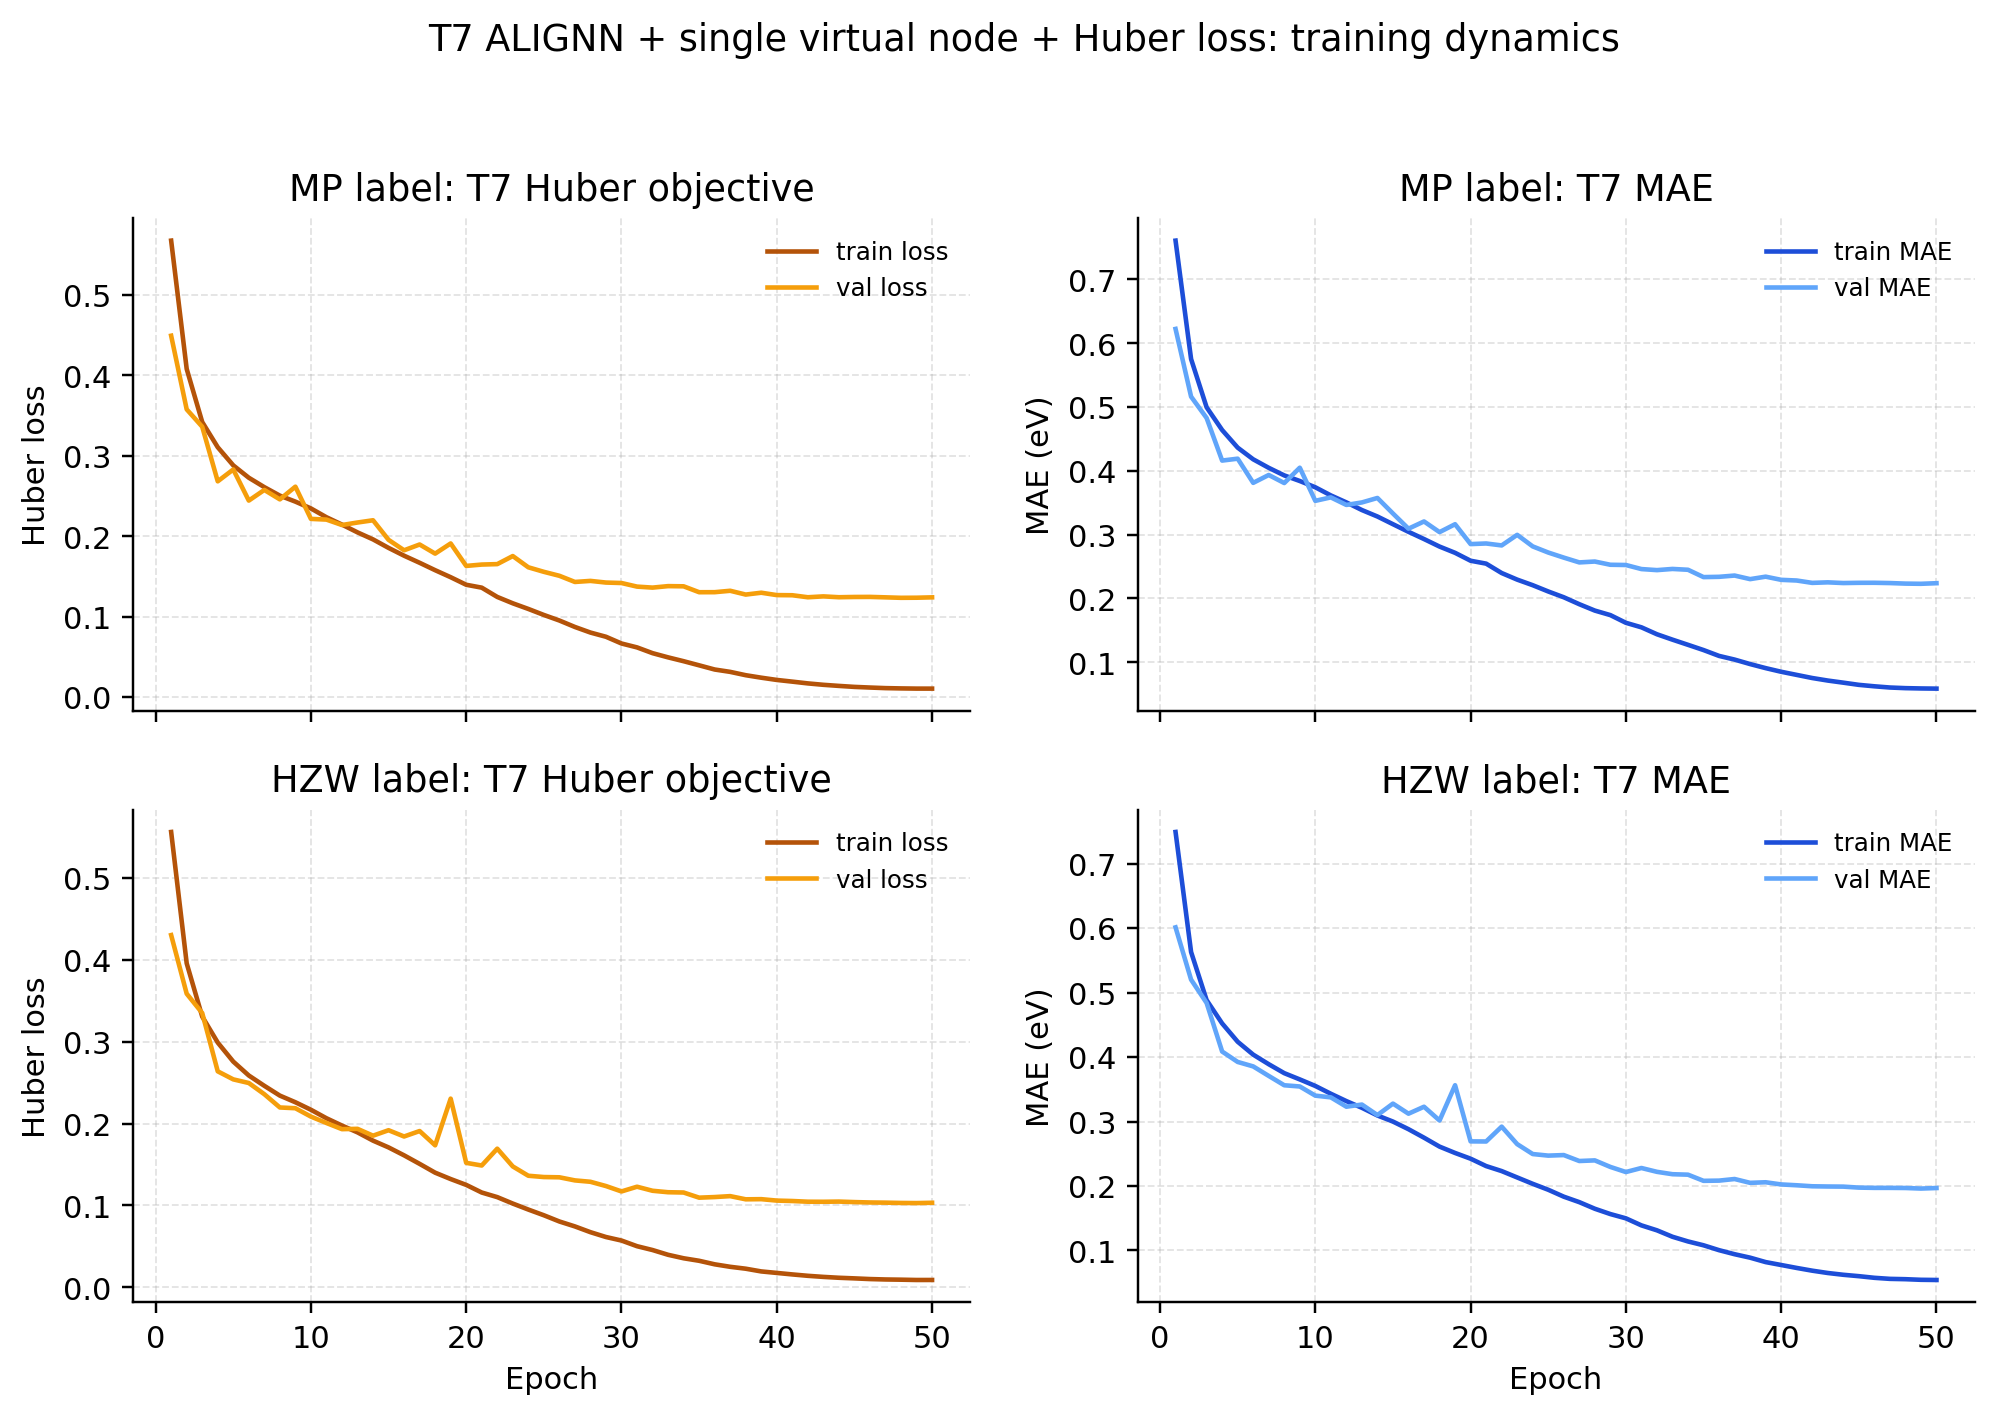
\includegraphics[width=\textwidth]{figures/huber_diagnostics/t7_huber_training_curves.png}
\caption{T7 Huber-only 消融的训练动态。左列为 Huber objective，右列为 MAE；上行为 MP label，下行为 HZW label。}
\label{fig:huber-training}
\end{figure}

\begin{figure}[htbp]
\centering
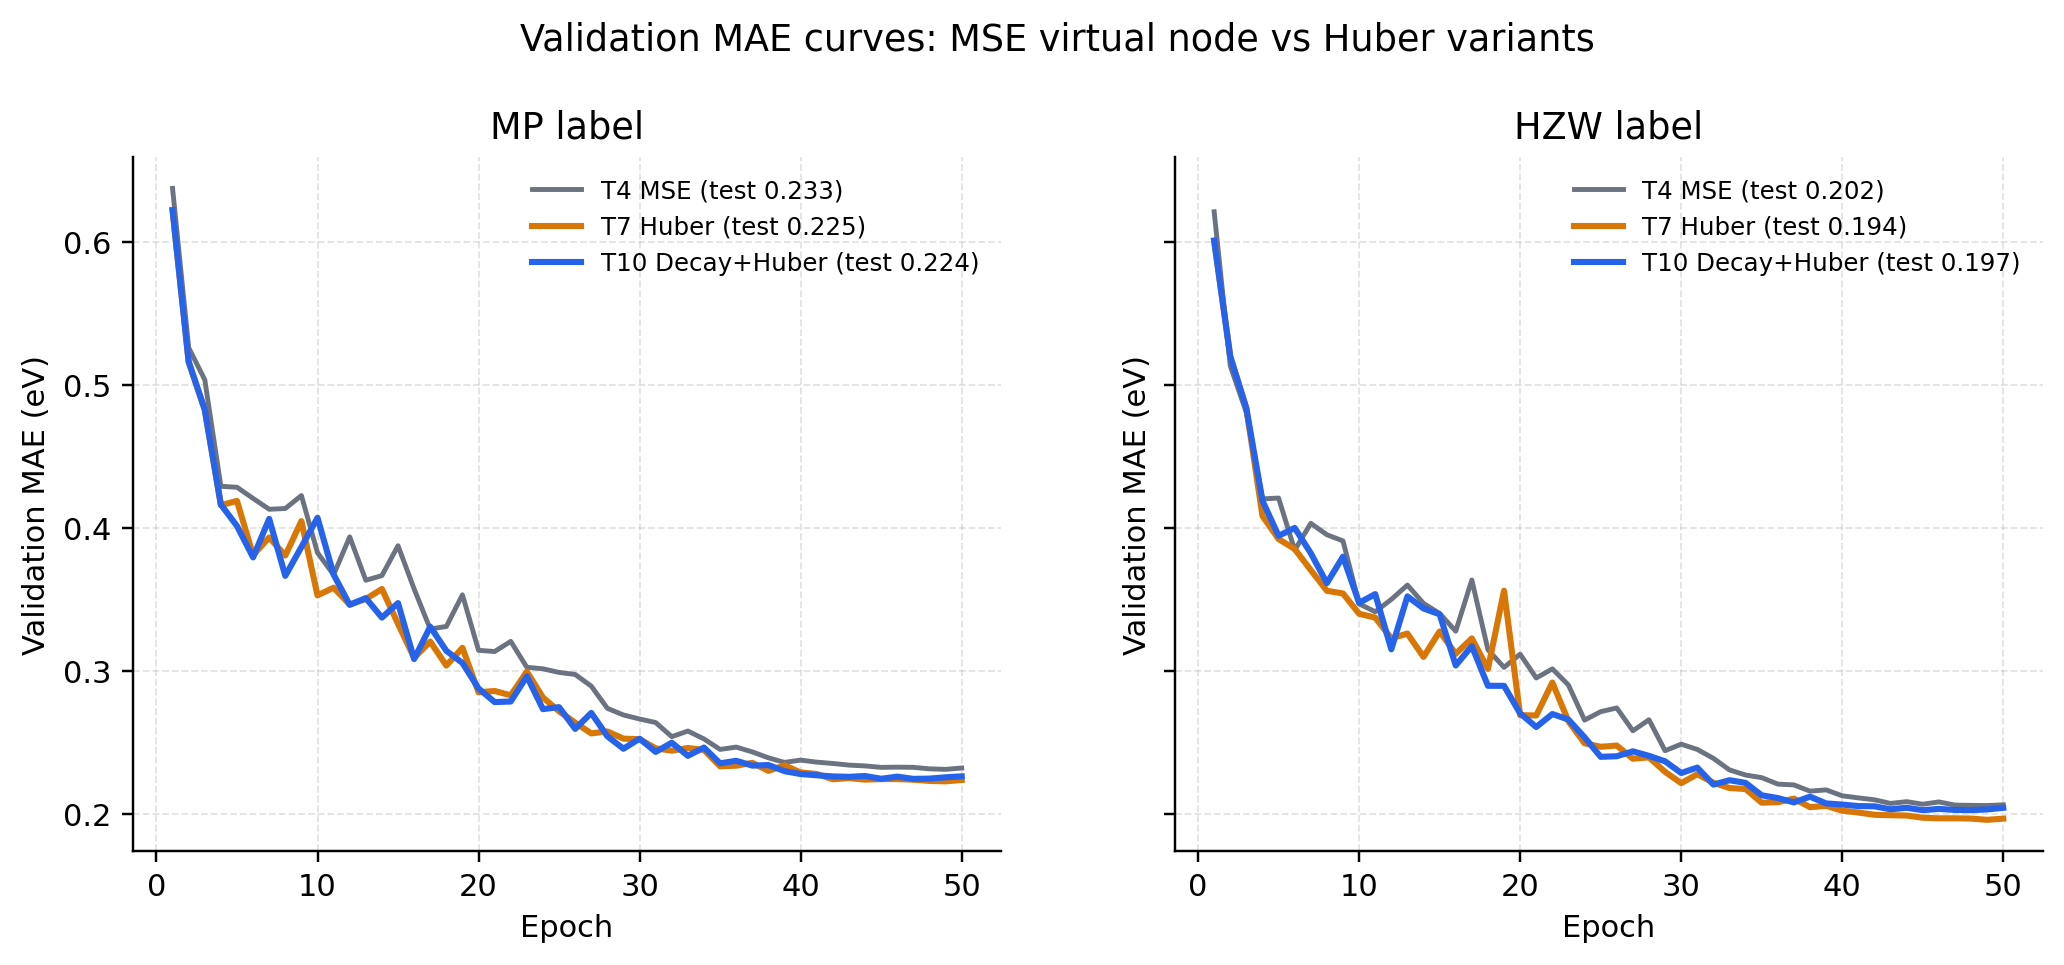
\includegraphics[width=\textwidth]{figures/huber_diagnostics/val_mae_curves_t4_t7_t10.png}
\caption{T4、T7 与 T10 的验证 MAE 曲线。T7 是 Huber-only 消融，T10 是在 Huber 主干上加入 global broadcast decay。}
\label{fig:huber-val-mae}
\end{figure}

\begin{figure}[htbp]
\centering
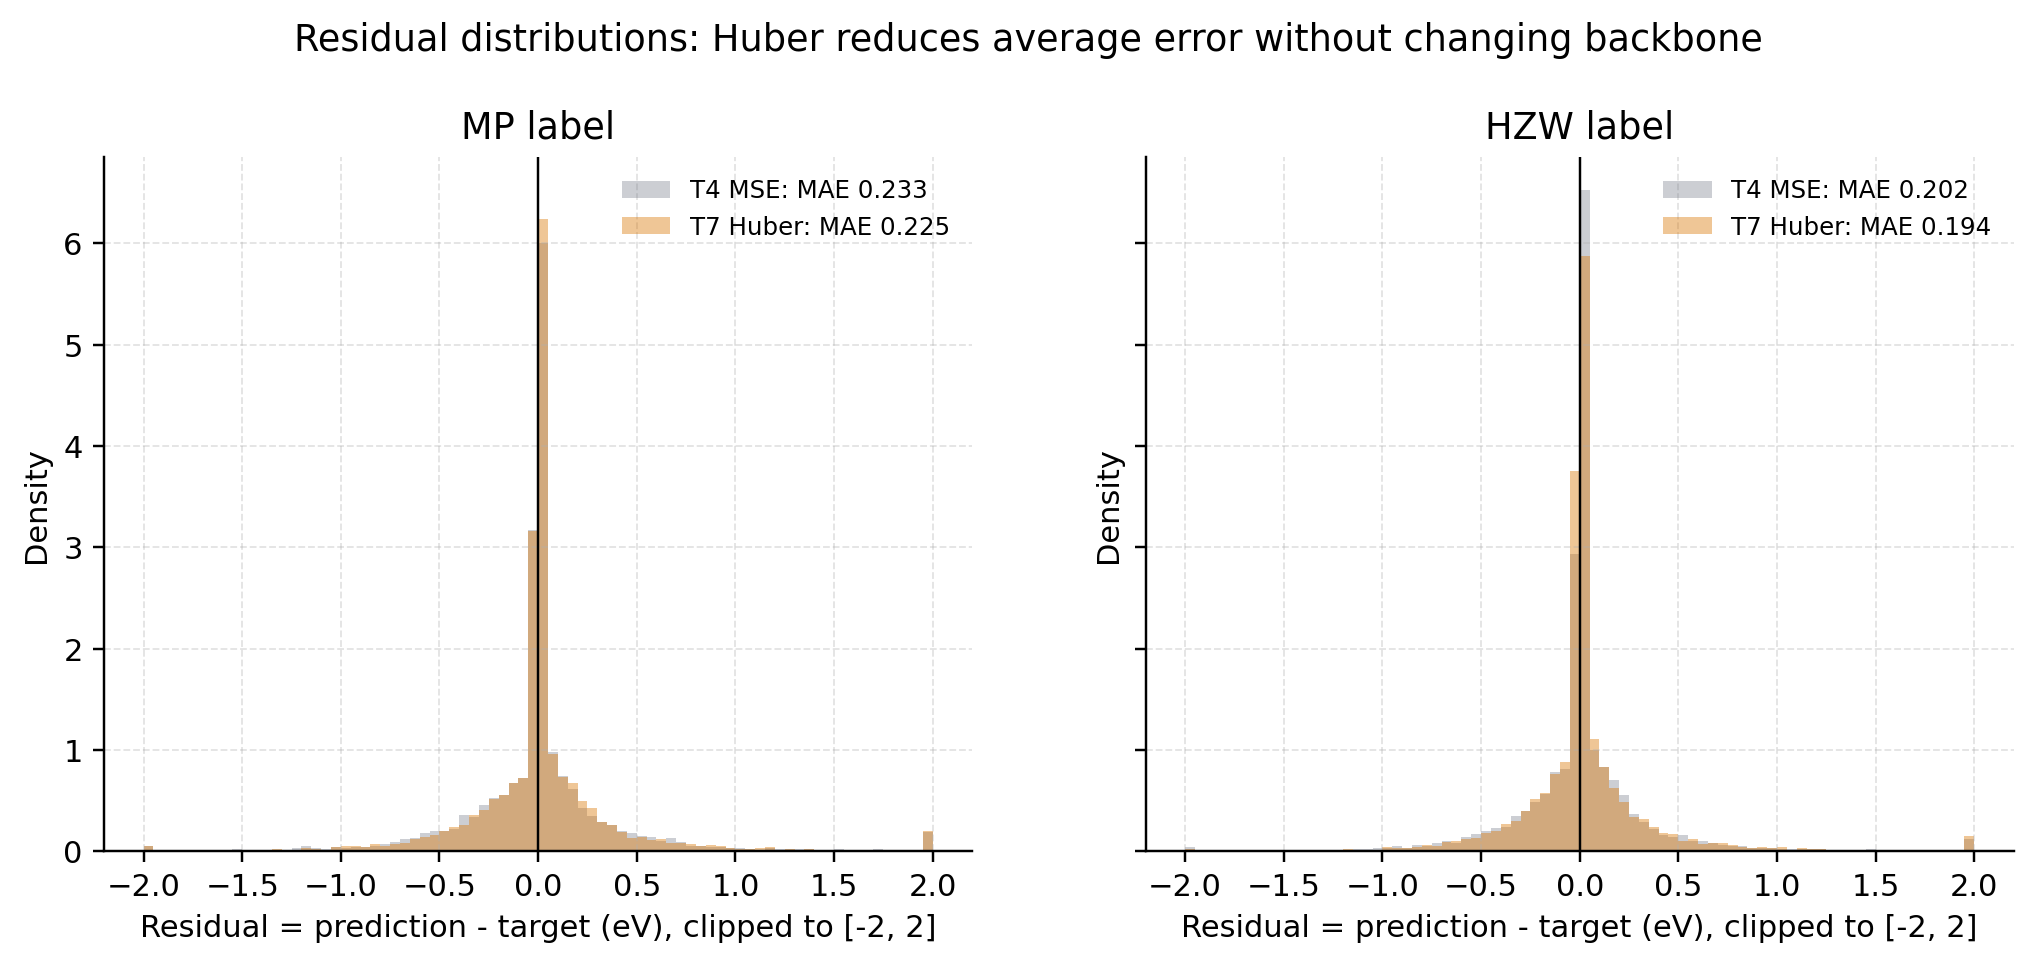
\includegraphics[width=\textwidth]{figures/huber_diagnostics/residual_hist_t4_vs_t7.png}
\caption{T4 与 T7 的测试集残差分布。残差定义为 $\hat{y}-y$，图中将残差截断到 $[-2,2]$ eV 以突出主体分布。}
\label{fig:huber-residual}
\end{figure}

\begin{figure}[htbp]
\centering
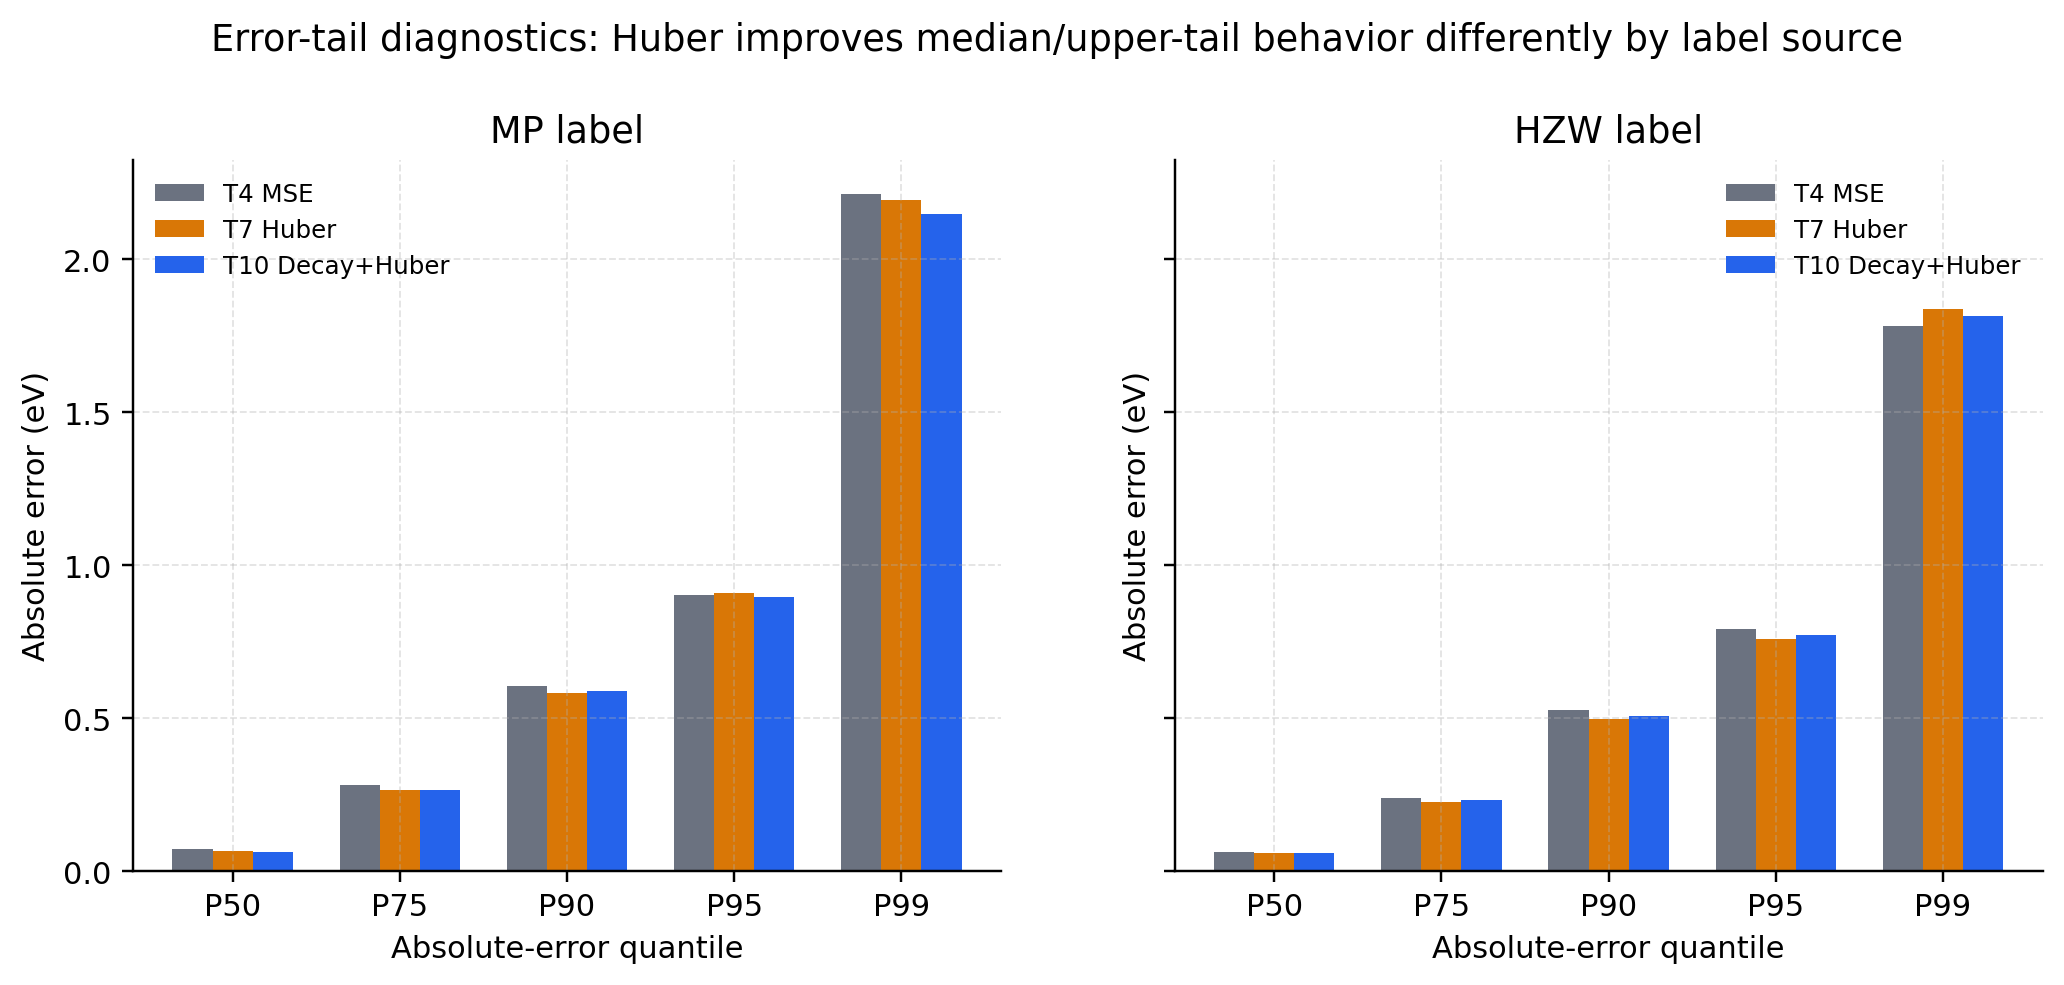
\includegraphics[width=\textwidth]{figures/huber_diagnostics/abs_error_quantiles_t4_t7_t10.png}
\caption{T4、T7 与 T10 的绝对误差分位数。该图用于观察 Huber 和 broadcast decay 对中位误差与长尾误差的影响。}
\label{fig:huber-quantile}
\end{figure}

\subsection{Top-$k$ 不是稳定主贡献}

Top-$k$ 的独立收益不稳定。MP label 中，T8 top-$k$-only 的 MAE 为 0.230402，略优于 T4 但明显弱于 T7；HZW label 中，T8 为 0.202603，反而弱于 T4。T6 与 T9 因同时含有 Huber，不能把收益单独归因于 top-$k$。因此本文不能把 top-$k$ 包装成最终成功机制，只能认为它是信息流调度探索的一部分。

\subsection{双节点和双槽位有局部价值但整体不稳}

HZW 早期 E8 分桶和 strict clean S13 分桶都显示，大结构可能受益于额外全局容量。然而，MP full、matched clean 和 S 系列整体结果都表明，双节点/双槽位并不是稳定主贡献。其困难在于：额外容量需要知道何时启用、学习什么职责，以及如何避免干扰中等结构上的局部精细拟合。当前 \texttt{num\_atoms} 代理变量和 always-on 双节点都不能稳定解决这个问题。

\subsection{数据源差异改变模型排序}

HZW 与 MP 的模型排序差异不能简单解释为训练不充分或 MP 结构更小。历史分析显示，MP 测试集大结构比例并不低于 HZW；E12 在 MP 上 second slot 也并未完全塌缩。更合理的解释是，HZW band gap 与 MP summary band\_gap 的标签体系差异改变了模型学习目标。MP--HZW structure-first audit 进一步证明，对应结构内部仍存在金属/非金属冲突和同类大数值差异。因此，材料 GNN 比较必须在表格标题、正文和结论中写明 label source。

\section{局限性}

第一，本文结果主要集中在 band gap 任务。Band gap 很大程度受局部化学环境、成键模式和电子结构计算口径影响，不一定是最能体现长程全局依赖的材料性质。因此，双槽位和全局 attention 在介电、压电、声子或输运性质上是否更有价值，需要单独实验。

第二，MP/HZW 标签冲突虽然被系统审计，但最终 relaxed clean equal-atoms 仍保留同类大数值差异样本。这样做提高了样本覆盖，但也意味着模型训练目标仍包含标签源噪声。Huber 的稳定收益可能部分来自对这些冲突样本的鲁棒性。

第三，当前表格主要来自单次固定划分训练，缺少多随机种子均值与置信区间。对于 T7 与 T10 这类差距较小的比较，未来应补充多 seed、bootstrap 或 paired error analysis。

第四，硬阈值路由和 test-only diagnostic 只能说明潜在方向，不能作为正式模型结果。后续若继续探索大结构专家，应使用 validation-selected threshold 或端到端可训练路由，并在 held-out test 上一次性评估。

\section{结论}

本文整理了晶体 band gap 预测项目从 E1--E13 模型增强、MP--HZW 数据审计，到最终 S/T 系列验证的完整实验主线。结果表明，ALIGNN 是最强传统 baseline；single plain virtual node 在 HZW、MP full 和最终 relaxed 双标签源中均是稳定增强；进一步加入 Huber loss 是跨 MP label 与 HZW label 最稳定的收益来源。

在最终 relaxed clean equal-atoms 口径下，MP label 上 T10 取得最低 MAE 0.223686，HZW label 上 T7 取得最低 MAE 0.194002。考虑跨标签源稳定性，本文建议把 T7，即 ALIGNN + single plain virtual node + Huber loss，作为当前主模型结论。T10 可以作为 MP label 特化改进，但不应被表述为跨源通用最优。

同时，top-$k$、warmup、broadcast decay、双节点和双槽位机制提供了有价值的诊断信息，但不是当前稳定主贡献。尤其是双节点在大结构上有局部信号，却在整体上经常被中等结构损失抵消。未来工作应围绕更可靠的样本级路由监督、多性质任务验证和多随机种子评估展开。

\appendix

\section{E1--E13 实验谱系}

\begin{longtable}{p{1.4cm} p{4.2cm} p{6.2cm} p{3.2cm}}
\caption{E 系列可引用主线谱系与论文定位。}
\label{tab:e-lineage}\\
\toprule
编号 & 模型 & 核心意义 & 论文定位 \\
\midrule
\endfirsthead
\toprule
编号 & 模型 & 核心意义 & 论文定位 \\
\midrule
\endhead
E1 & CGCNN & 晶体图卷积 baseline。 & 基线 \\
E2 & ALIGNN & 原子图 + line graph，显式键角建模。 & 最强传统 baseline \\
E3 & M3GNet & 三体几何材料 GNN。 & 对照 baseline \\
E4 & ALIGNN + single plain virtual node & 加入朴素全局超节点。 & 第一条稳定有效增强 \\
E5 & ALIGNN + Transformer & 全局注意力 only。 & 负例/不稳定增强 \\
E6 & ALIGNN + physics constraint & CBM/VBM 辅助监督和 gap 一致性。 & 物理约束尝试 \\
E7 & ALIGNN + 1 attentive virtual node & 单注意力超节点。 & HZW 上明显负优化 \\
E8 & ALIGNN + 2 attentive virtual nodes & 双注意力超节点。 & HZW 大结构有收益 \\
E9/E10 & size-aware / active size-aware gate & 显式尺度 gate 控制第二槽位。 & 历史探索 \\
E11 & hard/val routed ensemble & 小结构 E4、大结构 E8 的路由组合。 & 融合诊断，不是端到端模型 \\
E12 & size-supervised dual slot & size 不进前向，只进 loss 监督第二槽位。 & HZW 有效，MP 不稳 \\
E13 & E12 + physics & 双槽位 + 有效 mask 物理约束。 & HZW 历史最优 \\
\bottomrule
\end{longtable}

\section{T 系列定义与可引用状态}

\begin{longtable}{p{1.3cm} p{5.0cm} p{5.6cm} p{3.0cm}}
\caption{最终 T 系列定义。}
\label{tab:t-definitions}\\
\toprule
编号 & 模型 & 变更点 & 可引用状态 \\
\midrule
\endfirsthead
\toprule
编号 & 模型 & 变更点 & 可引用状态 \\
\midrule
\endhead
T1 & CGCNN baseline & 基础晶体图卷积。 & MP/HZW 主表可引用 \\
T2 & ALIGNN baseline & 最强传统 baseline。 & MP/HZW 主表可引用 \\
T3 & M3GNet baseline & 材料图 baseline。 & MP/HZW 主表可引用 \\
T4 & ALIGNN + single plain virtual node & 稳定全局超节点。 & MP/HZW 主表可引用 \\
T6 & ALIGNN + top-$k$ virtual node + Huber & 稀疏 node-to-global + 鲁棒损失。 & MP/HZW 主表可引用 \\
T7 & ALIGNN + single plain virtual node + Huber & Huber-only 消融。 & MP/HZW 主表可引用；跨源最稳 \\
T8 & ALIGNN + top-$k$ virtual node + MSE & top-$k$-only 消融。 & MP/HZW 主表可引用 \\
T9 & ALIGNN + warmup top-$k$ + Huber & 先 mean pooling，再逐渐打开 top-$k$。 & MP/HZW 主表可引用 \\
T10 & ALIGNN + global broadcast decay + Huber & 训练后期降低 global-to-node 广播。 & MP/HZW 主表可引用；MP label 最优 \\
\bottomrule
\end{longtable}

\section{结果来源路径}

\begin{itemize}
  \item 交付计划：\path{docs/plans/2026-06-11-latex-ppt-and-paper-deliverables.md}。
  \item HZW 早期报告：\path{gnn_project_history_report.tex}，\path{matbench_gnn_final_report.tex}。
  \item MP/HZW 诊断文档：\path{docs/2026-04-19-global-attention-vs-virtual-node.md}，\path{docs/2026-04-25-mp-vs-hongzhiwei-analysis.md}。
  \item Structure-first audit：\path{results/data_quality/structure_first_strict_180/}。
  \item Strict clean metadata：\path{results/data_quality/final_clean_mp/metadata.json}。
  \item S 系列分桶：\path{results/mp_hzw_final_clean_equal_atoms_mp_s/analysis/s4_vs_s13_size_analysis.md}。
  \item 最终 T 系列：远端 \path{/data/home/tg100025/gnn_work/results/mp_hzw_relaxed_clean_equal_atoms_mp_t/comparison_summary.csv} 与 \path{/data/home/tg100025/gnn_work/results/mp_hzw_relaxed_clean_equal_atoms_hzw_t/comparison_summary.csv}，数值已写入 2026-06-11 交付计划。
\end{itemize}

\begin{thebibliography}{9}

\bibitem{xie2018cgcnn}
Tian Xie and Jeffrey C. Grossman.
\newblock Crystal Graph Convolutional Neural Networks for an Accurate and Interpretable Prediction of Material Properties.
\newblock \emph{Physical Review Letters}, 120(14):145301, 2018.

\bibitem{choudhary2021alignn}
Kamal Choudhary and Brian DeCost.
\newblock Atomistic Line Graph Neural Network for improved materials property predictions.
\newblock \emph{npj Computational Materials}, 7:185, 2021.

\bibitem{chen2022m3gnet}
Chi Chen and Shyue Ping Ong.
\newblock A universal graph deep learning interatomic potential for the periodic table.
\newblock \emph{Nature Computational Science}, 2:718--728, 2022.

\bibitem{jain2013mp}
Anubhav Jain, Shyue Ping Ong, Geoffroy Hautier, Wei Chen, William Davidson Richards, Stephen Dacek, Shreyas Cholia, Dan Gunter, David Skinner, Gerbrand Ceder, and Kristin A. Persson.
\newblock Commentary: The Materials Project: A materials genome approach to accelerating materials innovation.
\newblock \emph{APL Materials}, 1:011002, 2013.

\bibitem{dunn2020matbench}
Alexander Dunn, Qi Wang, Alex Ganose, Daniel Dopp, and Anubhav Jain.
\newblock Benchmarking materials property prediction methods: the Matbench test set and Automatminer reference algorithm.
\newblock \emph{npj Computational Materials}, 6:138, 2020.

\bibitem{huber1964robust}
Peter J. Huber.
\newblock Robust Estimation of a Location Parameter.
\newblock \emph{The Annals of Mathematical Statistics}, 35(1):73--101, 1964.

\end{thebibliography}

\end{document}
